\documentclass[12pt]{article}

\usepackage{enumitem}
\usepackage[right=20mm, left=20mm]{geometry}
\usepackage{type1cm}
\usepackage{amssymb}
\usepackage[fleqn]{amsmath}
\usepackage{tikz}
\usepackage{multicol}
\usepackage{makecell}
\setlength{\columnsep}{1pt}
\usepackage{pgfplots}
\usepackage{float}
\usepackage{caption}
\usepackage{subcaption}
% \usepackage{subfig}
\usepackage{graphicx}

\usepackage{indentfirst}
\usepackage{lastpage}  
\usepackage{fancyhdr}
\pagestyle{fancy}

\usepackage{pgfgantt}

\usepackage[unicode=true,pdfusetitle,
 bookmarks=true,bookmarksnumbered=false,bookmarksopen=false,
 breaklinks=false,pdfborder={0 0 1},backref=false,colorlinks=false]
 {hyperref}

\makeatletter
\newenvironment{myalign*}{\ifvmode\else\hfil\null\linebreak\fi
  \hspace*{-\leftmargin}\minipage\textwidth
  \setlength{\abovedisplayskip}{0pt}%
  \setlength{\abovedisplayshortskip}{\abovedisplayskip}%
  \start@align\@ne\st@rredtrue\m@ne}%
{\endalign\endminipage\linebreak}

% Paper size
\topmargin -10mm
\textwidth 170mm
% \oddsidemargin -5mm
% \evensidemargin -5mm
\textheight 220mm

% Font setting
\usepackage{xeCJK}
% \setCJKmainfont{Noto Sans TC}
\setCJKmainfont{kaiu.ttf}


\renewcommand{\footnotesize}{\normalsize} 
\renewcommand{\headrulewidth}{0pt}
\renewcommand{\footrulewidth}{0pt}

\lhead{}
\chead{2023年全國大專校院智慧創新暨跨域整合創作企劃書}
\rhead{}

\lfoot{}
\cfoot{}
\rfoot{ 共 \pageref{LastPage} 頁 第  \thepage   頁} 

\makeatletter
\begin{document}
% \fontsize{14pt}{18pt}\selectfont
% \author{}
\date{}
\usetikzlibrary{automata, positioning, arrows}
% \maketitle
\tikzset{every state, accepting/.style={double distance=2pt}}
\captionsetup[figure]{labelfont={bf},name={圖},labelsep=period}

\noindent
\textbf{參賽隊名:} 普羅程式 \\
\textbf{作品名稱:} 威力導師 PowerTeacher \\

\begin{enumerate}
  \setlength{\parindent}{2em}
  \item 競賽主題:數位永續科技組 
  \item 創作主題
    \begin{enumerate}
      \setlength{\parindent}{2em}
      \item 題目
        \par TEMPLATE-ENUMERATE-CONTENT
      \item 實用功能描述
      \item 作品與市場相關產品差異
    \end{enumerate}
  \item 創意構想
    \begin{enumerate}
      \item 理論基礎
      \item 設計創新說明
      \item 特殊功能描述
    \end{enumerate}
  \item 系統架構
    \begin{enumerate}
      \item 架構說明
      \item 「人機介面設計」(UI)與「使用者體驗」(UX)設計
    \end{enumerate}
  \item 計劃管理
    \begin{table}[htb]      
      \centering
      \begin{tabular}{|c|c|c|}
        \hline
        \thead{工作階段} & \thead{工作日數} & \thead{工作內容} \\ \hline
        1 &  &  \\ \hline
      \end{tabular}
      \caption{計劃管理}
    \end{table}
    \begin{figure}[htb]
      \centering
      \begin{ganttchart}[
        y unit title=0.6cm,
        y unit chart=0.7cm,
        x unit=0.7cm,
        vgrid,hgrid, 
        title height=1,
        progress label text={},
        bar height=0.8,
        bar top shift=0.1,
        ]{1}{8}
        %labels
        \gantttitle{1}{1} 
        \gantttitle{2}{1} 
        \gantttitle{3}{1} 
        \gantttitle{4}{1} 
        \gantttitle{5}{1}
        \gantttitle{6}{1}
        \gantttitle{7}{1}
        \gantttitle{8}{1} \\
        
        %tasks
        \ganttbar{工作階段 1}{1}{2} \\
        \ganttbar{工作階段 2}{3}{4} \\
        \ganttbar{工作階段 3}{5}{6} \\
        \ganttbar{工作階段  4}{7}{8}
        % \ganttbar[progress=0]{工作階段  4}{7}{8}
      
        %relations 
        % \ganttlink{elem0}{elem1} 
      \end{ganttchart}
      \caption{甘特圖}  
    \end{figure}
  \item 修改舊作參賽說明
    \par 本專案開發之作品未使用團隊成員曾獲競賽獎勵之作品。
  \item 軟體清單
    \begin{enumerate}
      \item 作業系統環境:Windows、Linux
      \item 主要開發程式語言:Javascript、Golang
      \item 專案支援語言:中文
      \item 開發環境:
        \begin{enumerate}
          \item Visual Studio Code
          \item Node.js
          \item Node Package Manager
          \item Vue 3 Frontend Framework
          \item Gin Backend Framework
          \item Git, Github
        \end{enumerate}
      \item 專案成果預定授權條款:
        \par 本專案開發產品授權條款使用 CC BY-NC 4.0 宣告。
    \end{enumerate}
  \item 權力分配
    \par 依著作權法第 40 條之規定,由參賽學生與指導教授均等共有。

  % \begin{figure}[htb]
  %   \centering
  %   \begin{subfigure}{0.45\linewidth}
  %     \centering
  %     \href{https://raw.githubusercontent.com/programingtw/proglearn-plan/main/img/arc1.jpg}{
  %       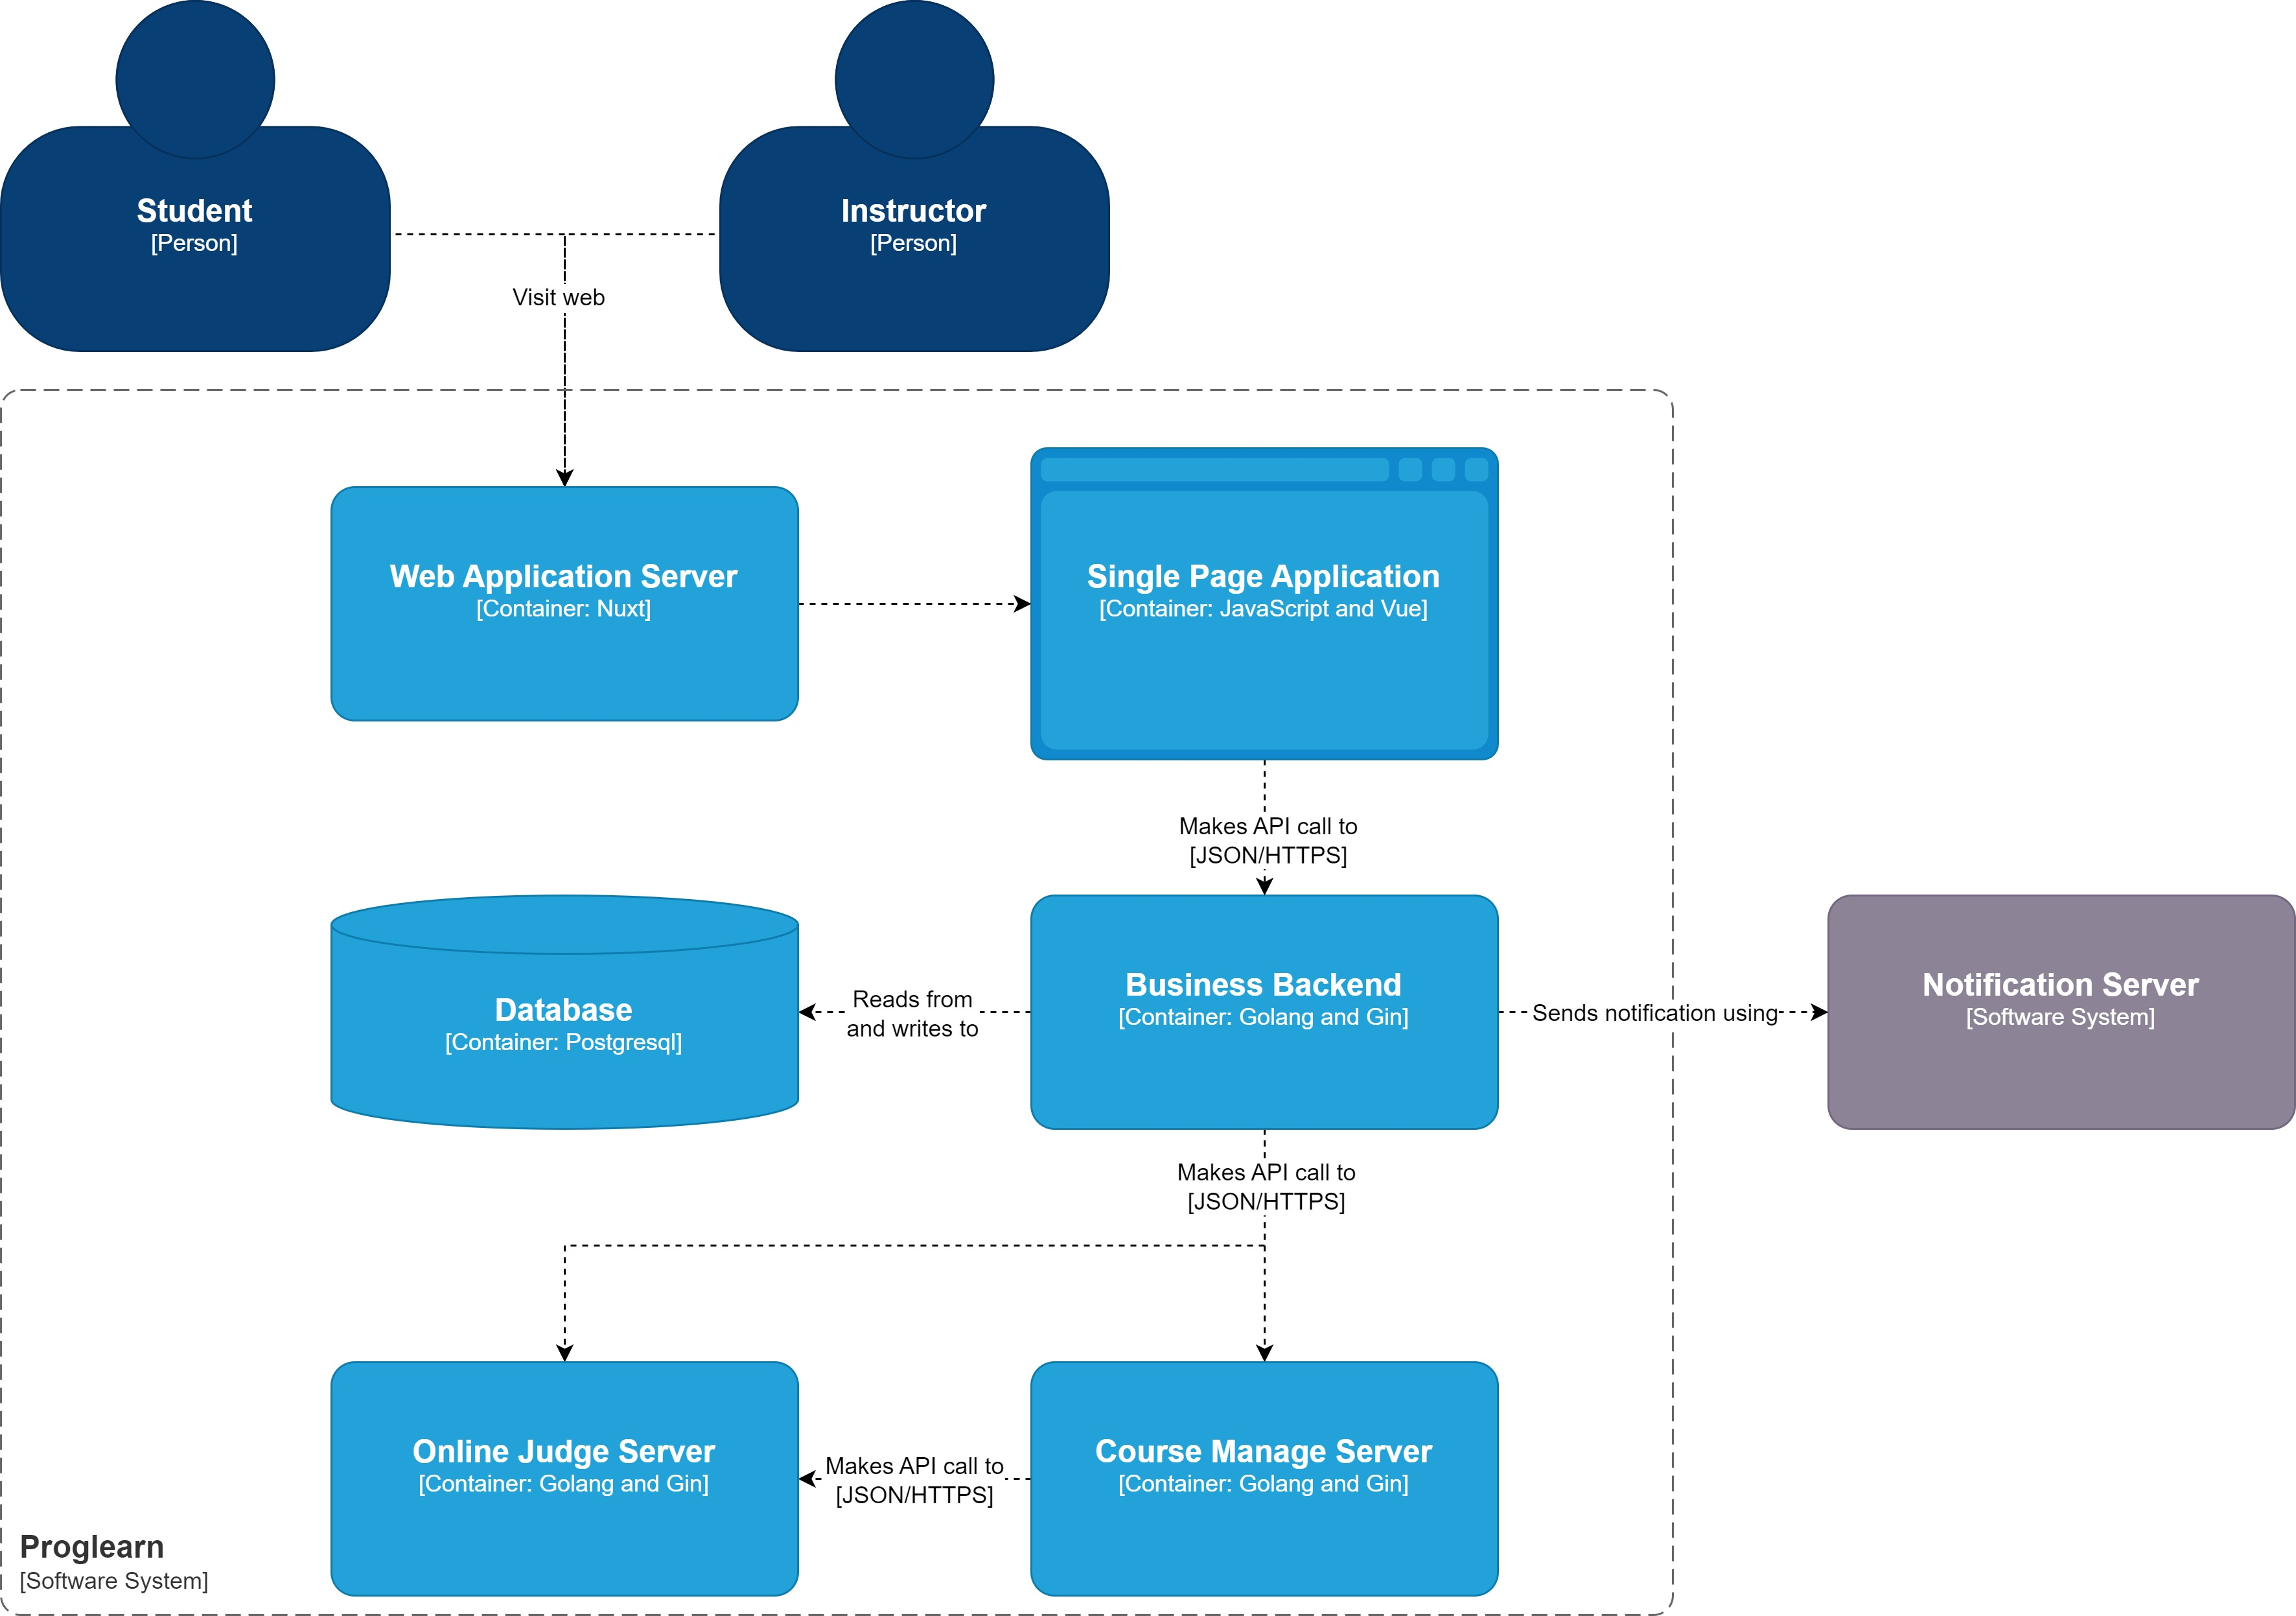
\includegraphics[width=0.65\textwidth]{./img/arc1.jpg}
  %     }
  %     \caption{CAPTION}
  %     \label{arc1}            
  %   \end{subfigure}
  % \end{figure}
\end{enumerate}
\end{document}
